%% Macromolecules manuscript draft (ACS achemso template, journal=mamobx).
%% Drafted 2026-10-19 (abstract, introduction, methods); results, discussion and conclusions 2026-10-21.
%% Revised 2026-10-27: methods and extended results moved to si.tex; ontology refinement (Part C) and the released
%% code (0.13.0) added.
%% Numbers come from the frozen knowledge base KF and the study's result sections (study plans at
%% main 6f25730), the ontology refinement plan, and the confirmation plan, or from the pinned code (tags
%% study-freeze-2, study-freeze-3, study-freeze-4). \tbd{} marks author actions.
%% See NOTES.md beside this file.
\PassOptionsToPackage{hyphens}{url}
\documentclass[journal=mamobx,manuscript=article]{achemso}

\usepackage{graphicx}
\usepackage{booktabs}
\usepackage{siunitx}
\usepackage{xcolor}
\usepackage{url}

%% Single-spaced throughout; the class double-spaces manuscripts.
\AtBeginDocument{\singlespacing}
%% No space above the title, and a wider abstract, so that the abstract and the AI statement fit on the first page.
\makeatletter\setlength\acs@space@pre@title{-3\baselineskip}\makeatother
\AddToHook{env/abstract/begin}{\setlength\leftmargini{1em}}

%% The Macromolecules configuration leaves sections unnumbered; numbered headings let the text say "Section 2.3".
\SectionNumbersOn

%% Draft-only marker for results that are not in yet. Remove before submission.
\newcommand{\tbd}[1]{\textcolor{red}{[#1]}}
\newcommand{\code}[1]{\texttt{#1}}
%% Release and prompt identifiers: monospaced, breakable at hyphens.
\newcommand{\ident}[1]{\path{#1}}

%% OOPC mark: the wordmark at the bottom right of every page, flush with the text's right edge and centred on the page
%% number's line. On every build since 2026-10-29 (owner); preprint.tex gives the same document. For a submission
%% without the mark, delete the \providecommand and the hook below.
\providecommand\OOPCpreprint{
\includegraphics[height=.17in]{figures/oopc-wordmark-paper}}
\AddToHook{shipout/foreground}{%
  \put(\dimexpr1in+\oddsidemargin+\textwidth\relax,\dimexpr-1in-\topmargin-\headheight-\headsep-\textheight-\footskip\relax)
    {\makebox[0pt][r]{\raisebox{\dimexpr.35em-.5\height\relax}{\OOPCpreprint}}}}

\author{Brett M. Savoie}
\email{bsavoie2@nd.edu}
\affiliation[University of Notre Dame]
{Department of Chemical and Biomolecular Engineering, University of Notre Dame, Notre Dame, Indiana 46556, United States}
%% \tbd{co-authors and affiliations}

\title{Open Ontology of Polymer Chemistry: Accumulation and Self-Improving Memory Mechanisms for Polymer Research}
%% Alternative working title: A Self-Improving Open Ontology of Polymer Chemistry

\abbreviations{DMA, DSC, LLM, OOPC, Tg, WOP}
\keywords{polymer informatics, ontology, provenance, language-model agents, literature research, polymer property data}

\begin{document}

\begin{tocentry}
%% TOC graphic: 3.25 in x 1.75 in, a reduced version of Figure 1.
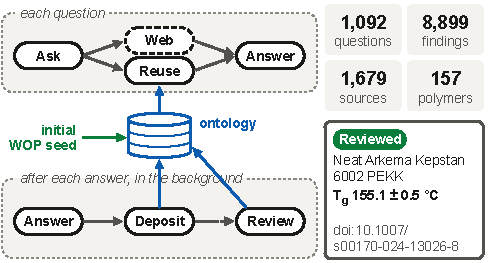
\includegraphics{figures/toc}
\end{tocentry}

%% ---------------------------------------------------------------------------------------------
\begin{abstract}
Memory systems for AI agents are a valuable component of long-running workflows.
They are also a strong form of lock-in for model providers, because the memory system that makes a model better with use may be inaccesible to users.
An ideal memory system would accumulate both factual knowledge and the relationships of that knowledge to recurring tasks performed by the researcher.
People accumulate particular and general knowledge through experience, the latter often through periodic reflection on what is working and isn't working at a higher level of abstraction.
Here, we introduce an open-source harness for polymer research meant to heuristically mimic (i) knowledge accumulation across research tasks, (ii) the review of new knowledge against existing knowledge, and (iii) performing periodic updates to task-knowledge relationships through reflection.
The system, which we call the Open Ontology of Polymer Chemistry (OOPC, pronounced `oopsie'), is initialized with a knowledge base consisting of an open-source wikipedia with entries for most known polymers.
From this starting point, the knowledge base was enriched by running a 1,092 task campaign across different areas of polymer chemistry, producing 8,899 distinct findings extracted from 1,679 sources on 157 different polymers.
GPT-6.1 Sol and Opus 5.5 comparisons were run with and without the accumulated memory from this campaign on 60 held-out tasks with varying overlap in terms of polymer and properties being researched.
The performance improvements tracked with research topic similarity to prior work researched from the harness, with token reductions of up to 19\% and 48\% and web search reductions of up to 80\% and 72\% (10.3 to 2.1 and 7.6 to 2.1 per answer) for Opus 5.5 and GPT-6.1 Sol, respectively.
The harness was tested through five independent restarts of 500 tasks each with reproducible performance gains.
An independent review of the performance caught rare contradictory claims and occasionally unsubstantiated claims depending on the underlying model (up to a few percent of all claims by claude on withheld tasks, none by codex).
The reflection heuristic was tested as an update to the knowledge ontology after the accumulation period.
These updates mainly consisted of extended lists of property names with marginal improvements to finding recall. 
The roles of review and ontology updates require further study as after knowledge accumulation these tests had little room to show appreciable gains given the consistently strong evidentiary basis for findings within the harness.
Looking forward, domain-specific memory systems are likely to be valuable and ideally transferable research artifacts that can be shared at the group, community, and organizational levels.
\end{abstract}
%% 435 words, written by the owner (2026-10-29), above the 100-150 that an ACS guideline search gave
%% (unconfirmed; NOTES.md). Numbers: A2 and E8 near questions, KF against K0: Claude Code (Opus 5.5) tokens 0.81
%% (19%), web 10.3 -> 2.1 (80%); Codex (GPT-6.1 Sol) tokens 0.52 (48%), web 7.6 -> 2.1 (72%); Part B restarts, five
%% rounds of 100 tasks each; E8 contradicted 22 of 370 (K0) and 19 of 452 (KF) statements, Codex 0 of 982; Part C.

%% The owner's AI statement, kept after the abstract by the owner's choice (ACS asks for it in the acknowledgement).
{\small\itshape\noindent\textbf{AI Statement:} The abstract and conclusions were written by Brett, the rest of the manuscript is the result of multiple drafts between Opus 5.5 and 6.5-Sol with light editing from Brett.\par}

%% ---------------------------------------------------------------------------------------------
\section{Introduction}

Polymer property data underpin materials selection and, increasingly, data-driven polymer design.\cite{Audus2017Polymer,Chen2021Polymer}
Few of these data are properties of a repeat-unit structure alone.\cite{Jha2019Uncertainty,Liu2023Ontology}
A reported glass transition temperature belongs to a particular grade, molecular weight, and thermal history, measured by a particular method at a particular heating rate or frequency.\cite{FoxFlory1950Second,Hutchinson2009Glass,Jha2019Uncertainty}
An oxygen permeability likewise belongs to a film measured at a particular temperature and relative humidity.\cite{Muramatsu2003Oxygen,Mokwena2012EVOH}
Curated databases preserve this context by storing values together with their samples and measurement conditions,\cite{Otsuka2011PoLyInfo,Liu2023Ontology} but curation is labor-intensive,\cite{Tchoua2016Blending,Ma2020PI1M} and most published polymer data still reside in the text and tables of individual papers.\cite{Kononova2021TextMining,Shetty2023Pipeline}
Research agents built on large language models (LLMs) now plan and execute chemical tasks with web search and expert tools,\cite{Boiko2023Coscientist,Bran2024ChemCrow} and on some literature tasks they answer technical questions with citations at a level that matches or exceeds domain experts.\cite{Skarlinski2024PaperQA2}
Nevertheless, these agents treat every question as the first.
The sources they find and read are discarded when the session ends, together with the provenance needed to judge whether a reported value applies to a given material and set of conditions.

Two lines of work have begun to address the scale of the polymer literature.
The first extracts structured property records from published text in bulk.
Rule-based pipelines such as ChemDataExtractor established that materials data can be mined from text at scale,\cite{Swain2016ChemDataExtractor} and pipelines built on materials-specific language models and general-purpose LLMs have since extracted about 300,000 property records from polymer abstracts\cite{Shetty2023Pipeline} and more than one million from full-text polymer articles.\cite{Gupta2024LLM}
Conversational prompting with follow-up verification questions reaches precision and recall near 90\% on some materials data,\cite{Polak2024Extracting} and fine-tuned models and annotated corpora now link materials, properties, values, and conditions as structured relations.\cite{Dagdelen2024Structured,Cheung2024POLYIE}
The second line uses agents that plan searches, read full texts, and synthesize cited answers to individual questions.\cite{Lala2023PaperQA,Skarlinski2024PaperQA2}
Each line succeeds at its own task, but neither accumulates knowledge that later questions can build on.
Extraction pipelines run once over a fixed corpus and schema, decoupled from the questions researchers ask, and their records are seldom checked again against their sources.
Agents read sources in response to questions but keep nothing beyond the answer.

Memory is becoming a central component of agent systems, together with the harness, the tools, instructions, and stored files that wrap a model.
Research systems give agents memories of past interactions,\cite{Packer2023MemGPT,Park2023Generative} libraries of skills and workflows learned on earlier tasks,\cite{Wang2023Voyager,Wang2024Workflow} and reflections on their own failures,\cite{Shinn2023Reflexion} and frameworks for language agents now treat long-term memory as a module alongside reasoning and action.\cite{Sumers2024CoALA,Zhang2024Memory}
The harness alone can change what a fixed model achieves; a purpose-built interface, for example, raised a coding agent's success on real software issues.\cite{Yang2024SWEagent}
Commercial assistants now remember their users across conversations,\cite{OpenAI2024Memory,Anthropic2025Memory} but the provider holds that memory, and what can move to another assistant is a text summary of the user and past conversations.
A memory kept by the harness on the researcher's own machine, and read through an open tool standard such as the Model Context Protocol,\cite{Anthropic2024MCP} would instead stay with the researcher as models change.
Whoever holds them, retrieval stores and agent memories keep text or the agent's own reflections,\cite{Lewis2020RAG} not values carrying the material scope and conditions that make a polymer measurement interpretable.

Accumulation also creates a problem that a single answer does not have.
LLMs generate fluent statements that their sources do not support,\cite{Ji2023Survey} and in one audit 18\% of the citations that GPT-4 supplied for literature reviews were fabricated.\cite{Walters2023Fabrication}
An agent that reuses its own earlier output can propagate one such error into many later answers.
Scientific data infrastructures manage this risk through provenance.
The FAIR principles ask that data carry rich metadata and a traceable origin,\cite{Wilkinson2016FAIR} and the PROV ontology records which agent produced which entity from which source.\cite{Lebo2013PROVO}
Polymer data models such as BigSMILES and CRIPT give polymer identity and measurement context machine-readable forms,\cite{Lin2019BigSMILES,Walsh2023CRIPT} and ontologies for polymer nanocomposites and conjugated-polymer devices record sample provenance and process history.\cite{McCusker2020NanoMine,Liu2023Ontology}
These frameworks define what a trustworthy record looks like, but they presume a human curator or a validated pipeline to create each record and vouch for it.
It remains unresolved how a research agent should deposit what it reads.
Each value would need to keep its source, locator, and conditions; the party that vouched for it would need to be recorded; and a later question would need to distinguish a value checked against its source from one the agent merely read.

A related question is whether such a system can improve itself from its own records.
Automated prompt optimization has improved LLM performance on fixed benchmarks,\cite{Yang2023OPRO,Khattab2023DSPy,Yuksekgonul2025TextGrad} and self-improving agents now rewrite their own code against benchmark scores.\cite{Zhang2025Darwin}
These methods revise the agent's instructions or code rather than the vocabulary through which saved knowledge is found, and they have not been tested on open-ended literature research, where answers cannot be scored against a fixed key.
An accumulating ontology offers a second target for such revision, because each failed lookup is recorded in the agent's own traces.

Here, we report the Open Ontology of Polymer Chemistry (OOPC), an ontology that accumulates source-qualified polymer knowledge as a research agent answers questions (Figure~\ref{fig:overview}).
The ontology is seeded with 274 polymer identities from the Wiki of Open Polymer Data (WOP),\cite{WOP2026Wiki} which give every saved value a stable polymer to be filed under.
An open-source harness keeps the ontology and its findings on the researcher's machine and serves them to the agent through one search tool over the Model Context Protocol, so the same memory works with OpenAI's Codex and Anthropic's Claude Code.
Its memory rests on three mechanisms.
For accumulation, the researcher saves each value it reads as a finding with its material, property, value, unit, conditions, source, and locator, and a separate reviewer checks a defined subset against the sources.
For retrieval, a later question's search resolves polymer names through the ontology and returns the findings saved for that polymer's family, together with the method and specimen details saved from the same sources.
For reflection, model sessions read the loop's records and propose bounded edits to the researcher's instructions or to the ontology's names, annotations, and property terms, which are kept only if they pass fixed checks and, for the ontology, a reviewer session.
Over 1,092 questions, the loop built a knowledge base of 8,899 findings from 1,679 sources on 157 polymers, which we characterize as a polymer dataset in its own right.
On held-out questions near past work, the researcher used 0.52 of the tokens and 0.28 of the web calls that it needed with a 150-finding store, with no more contradicted statements, and the saving followed whether the question's own topic had been saved rather than the size of the store.
The store, written with Codex, also cut Claude Code's web calls from 10.3 to 2.1 per answer, although Claude Code's answers were less well supported with either store.
Reflection found real failures but changed answers little: adopted prompt edits changed cost by nothing measurable, and 148 ontology edits derived from answer traces raised search recall from 0.90 to 0.92 without changing cost on withheld questions.
Both tests left little room for a gain, because the development questions barely touched the store and the withheld questions' topics were already well covered.

\begin{figure*}
  \centering
  \singlespacing
  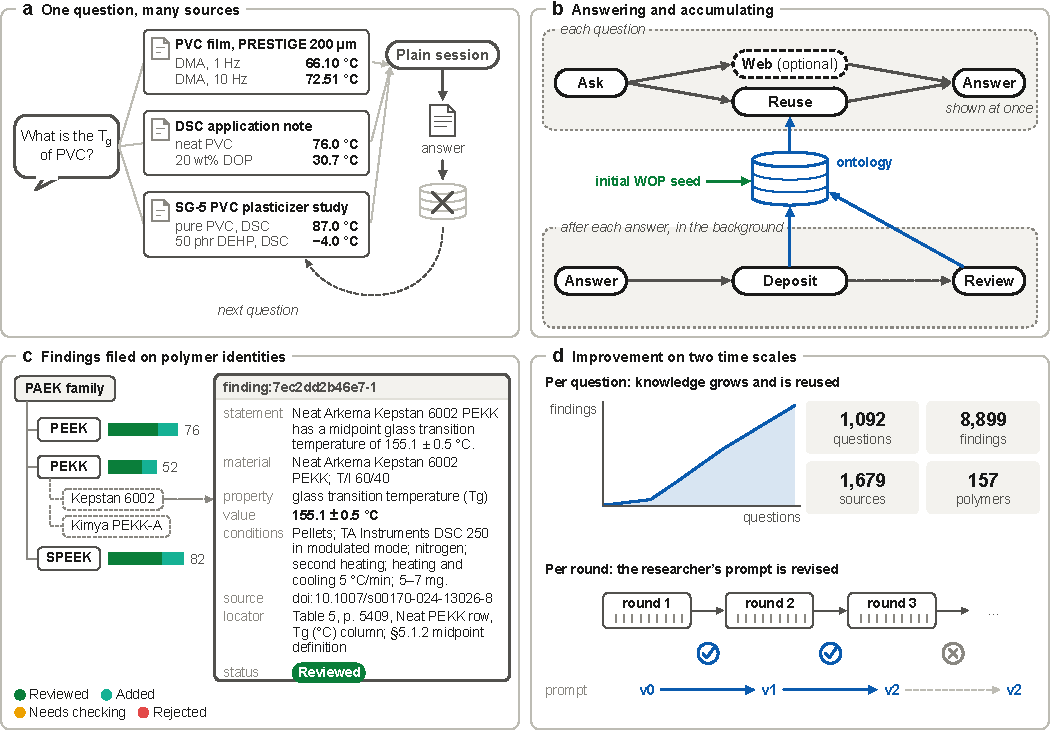
\includegraphics[width=\textwidth]{figures/fig1}
  \caption{An ontology that accumulates source-qualified knowledge.
  (a) One polymer property question draws on sources that differ by grade, specimen, method, and conditions, shown here as glass transition temperatures of poly(vinyl chloride) saved in the knowledge base from three sources; a plain agent rereads such sources for each question and keeps nothing.
  (b) Answering and accumulating around the ontology, as in the released code. For each question, the researcher reads saved findings first, uses the web only for what they lack, and answers, and the answer is shown at once. In the background, the same session then returns the findings and source notes it read, which are deposited as Added if read directly and as Needs checking if read off a figure, converted, or combined, and a reviewer session checks every finding that needs checking and one in five Added findings against their sources. The ontology starts from the polymer identities of the WOP seed.
  (c) Findings filed under polymer identities in the ontology, shown for the poly(aryl ether ketone) family with each polymer's findings as a bar colored by status and two grades as the findings name them (dashed), and one finding with its statement, material, property, value, unit, conditions, source, locator, and status.
  (d) Improvement on two time scales. Knowledge grows and is reused question by question, and the researcher's instructions are revised between rounds of questions, shown for an automated test of three rounds of 100 tasks (Section~S7), in which two of three proposed edits were adopted.
  Counts are those of the frozen knowledge base.}
  \label{fig:overview}
\end{figure*}

%% ---------------------------------------------------------------------------------------------
\section{Results and Discussion}
\label{sec:results}

\subsection{The Ontology and Its Research Loop}
\label{sec:loop}

An overview of the ontology and its research loop is provided here and in Figure~\ref{fig:methods} to guide the reader, and each component is described fully in the Supporting Information (Sections~S1--S7 and S11).
The ontology has two layers (Figure~\ref{fig:methods}a).
The seed layer holds 274 polymer concepts with stable identifiers, 245 structures, and 16,925 sourced claims imported one way from a pinned snapshot of WOP (Section~S1).
The knowledge layer holds what research produces.
Its unit is the finding, one source-qualified value comprising a one-sentence statement, the material as specifically as the source identifies it, the property, the value with its unit, the conditions as the source states them (specimen, processing history, method, and test conditions), the source with an exact locator, and a verbatim excerpt of at most about 25 words.
A source note records each source a session read, including sources that lacked what was sought or could not be opened.
Each finding carries one of four statuses.
\emph{Reviewed} findings were supported by a separate reviewer session, \emph{Added} findings were saved on the researcher's judgement, \emph{Needs checking} findings await review or could not be confirmed, and \emph{Rejected} findings were judged unsupported and are never returned by search.

\begin{figure*}
  \centering
  \singlespacing
  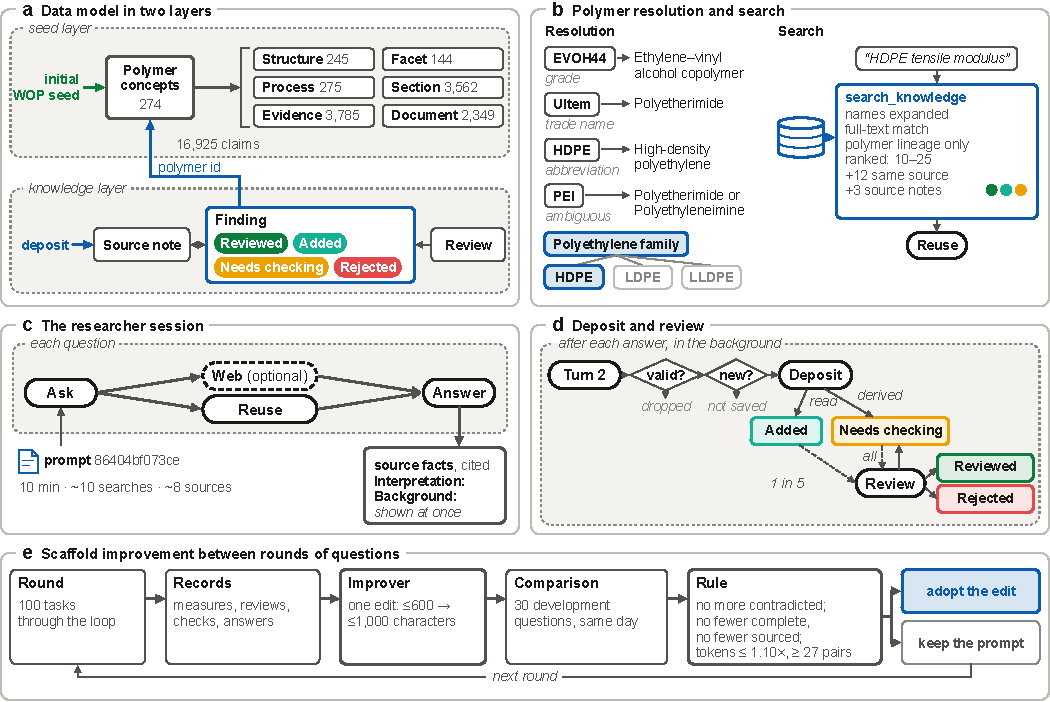
\includegraphics[width=\textwidth,height=0.55\textheight,keepaspectratio]{figures/fig2}
  \caption{The ontology and its research loop.
  (a) Data model in two layers: the seed layer of polymer concepts, structures, facets, processes, sections, evidence, and documents imported from WOP and linked by claims, and the knowledge layer of findings, source notes, and reviews.
  A finding is linked to the seed by its polymer identifier and to the source notes of its document by a source key.
  (b) Polymer resolution and search: names, grade designations, trade names, abbreviations, and family membership resolve to seed identities, and an abbreviation that names two polymers is returned to the asker. A search returns findings within the polymer's lineage (its families and members, not its siblings), ranked by query-word coverage with a limit of 10 to 25, followed by up to 12 findings saved from the same sources and up to three source notes, grouped by review status.
  (c) The researcher session, the each-question branch of Figure~\ref{fig:overview}b: one versioned prompt (the released prompt's hash is shown), saved knowledge first and the web for gaps under a depth budget (the standard depth is shown), and an answer with three kinds of statement, shown at once.
  (d) Deposit and review, the branch of Figure~\ref{fig:overview}b that runs in the background after each answer. In a second turn, the researcher session resumes to return the findings and source notes it read. A finding is saved if it is valid and new, as Added or Needs checking by how its value was obtained, and a reviewer session checks every finding that needs checking and one in five Added findings and returns Reviewed, Rejected, or Needs checking with a one-sentence reason.
  (e) Scaffold improvement between rounds of questions: the round's records, one proposed edit to the prompt, a same-day comparison of both prompts on development questions, and adoption by a fixed rule.}
  \label{fig:methods}
\end{figure*}

Accumulation begins with the researcher session (Figure~\ref{fig:methods}c; Section~S3).
Each question is answered by one non-interactive session of a subscription coding agent with live web search and one additional tool, \code{search\_knowledge}.
All experiments used OpenAI's Codex agent with the model gpt-6.1-sol for research, review, and checking unless stated otherwise, and Anthropic's Claude Code with the model claude-opus-5-5 proposed the prompt and ontology edits and scored the case studies blind.
The researcher's instructions are a single prompt, identified by a hash of its text and reproduced in Section~S16, which asks it to search saved knowledge before the web, to cite a saved finding rather than reopen its source, and to treat findings that need checking as leads to be confirmed.
An answer contains three kinds of statement.
A statement of what a source reports carries an inline citation to a finding or a source URL, the researcher's own reasoning begins with ``Interpretation:'' and cites its premises, and textbook background begins with ``Background:''.
The deposit rule makes the loop cumulative.
Every value that the answer reports from a source the session read is saved as a finding, together with up to about ten further values from the same passage that describe the same material or a closely related property, because reading them again later would cost another session.
Each finding also records whether its value was read in the text or a table, read off a figure, converted, or combined.
In the released code, the answer is shown at once and the same session then resumes in the background to return these findings and source notes (Figure~\ref{fig:methods}d; Section~S3.1), whereas in the frozen code of the experiments one turn returned the answer and its findings together.
A confirmation run on the released code reproduced the headline results of the frozen code, at about a quarter more new tokens per answer (Section~S12).

How a finding is vouched for depends on how its value was obtained (Figure~\ref{fig:methods}d; Section~S4).
A returned finding is saved only if it has a statement, a source, and a locator or an excerpt, and a fact is not saved twice.
A value the researcher read directly in the text or a table is Added on its judgement, and a value read off a figure, converted, or combined is Needs checking until reviewed.
After the answer has been delivered, the open copy of each cited source is captured without circumventing any access control, and one reviewer session checks every finding that needs checking together with a stable random sample of one in five Added findings.
The reviewer is a fresh session with web access but no access to the store, and it returns supported, unsupported, or uncertain with a one-sentence reason, which makes the finding Reviewed, Rejected, or Needs checking.
The verdict and reason stay with the finding, so a later answer can distinguish a value checked against its source from one the agent merely read.

Retrieval runs through the ontology rather than through text similarity alone (Figure~\ref{fig:methods}b; Sections~S2 and S5).
A polymer named in a query is resolved to a seed identity through names and aliases, grade designations, trade names, and family membership, so that EVOH44 resolves to ethylene vinyl alcohol copolymer and a search for high-density polyethylene reaches findings filed under the polyethylene family but not those filed under low-density polyethylene.
The query is matched against a full-text index of each finding's statement, material, property, conditions, source title, and excerpt, with each polymer name expanded by its other names in the seed.
Only findings filed under the resolved polymer, its broader families, or its narrower members are kept, ranked by the fraction of the query's other words they contain, and up to 12 further findings saved from the same sources follow.
These are usually the method, specimen, and conditions that accompany a value, so a source that has already been read need not be opened again.
Results are grouped by status, and every call is recorded with its exact returned payload, so whether a later session was shown a finding, and whether it cited the finding, are observed rather than inferred.

We test two reflection heuristics, each of which reads the loop's records, proposes bounded edits, and keeps them only if they pass fixed checks (Sections~S7 and S11).
The first revises the researcher's prompt between rounds of questions (Figure~\ref{fig:methods}e).
After each round of 100 questions, one model session without tools reads the round's records and proposes one edit that replaces a passage of at most 600 characters.
The current and proposed prompts then answer 30 fixed development questions, and the edit is adopted only if it gives no more contradicted statements, no fewer complete answers or sourced results, and a median paired token ratio of at most 1.10.
The second refines the ontology from answer traces, and in this study it was run once, as a separate study on the frozen knowledge base.
A deterministic miner replays every recorded knowledge search and classifies lookup failures as misses, in which the store held a finding that a search did not return, or as unnecessary hops, in which a web search and page open reached what the store already held.
A curator session reads the grouped failures and proposes edits from a closed list (names, polymers, family links, finding annotations, links between sources, and property terms), each citing the failures it answers.
A reviewer session approves or rejects each edit against its sources, and a replay of past searches drops any edit that loses more results than it fixes.
Neither heuristic can change a finding's statement, value, source, or status.
The harness now includes the second heuristic as an optional scheduled job, off by default, that proposes only names, polymer-identity annotations, and property terms, the kinds of edit the study produced, and writes the edits that pass these checks to a local overlay that search reads, which leaves the seed unchanged and lets each edit be reverted.

\subsection{Experimental Design}
\label{sec:design}

We characterize the knowledge base and measure what it buys through controlled experiments on a frozen copy, denoted KF (Sections~S6 and S9).
KF was built through the loop by 1,092 questions, comprising 92 earlier questions from development use, a 200-task observation run, and a campaign of 800 tasks in three waves whose question bank combined 135 polymers with properties, factors, or comparison groups suited to each polymer's class.
Because the prompt, the model, and the review policy changed between waves, the records of the build are analyzed descriptively.
K0, the 150-finding store left by development use before the build, serves as the low-knowledge reference.
The main experiments use 60 held-out questions in three strata of 20.
A near question asks about the polymer and property of a campaign question from another angle, a mid question asks about a well-covered polymer for a property never asked for it, and a far question asks about a polymer with no finding in its family.
Answers are judged for source support by an independent checker, a fresh session that reads each cited source and judges every substantive statement by its kind (Section~S8).
Quality is reported first through contradicted statements, complete answers, and answers giving a sourced result, and cost through new tokens (uncached input plus output), web calls, and time.
Comparisons between arms are paired by question, and relative cost is the median paired token ratio with a bootstrap 95\% interval over questions (Section~S14).
The checker judges source support rather than correctness, its verdicts are measurements with their own noise, and no human graded the answers.
Every experiment's predictions were committed before its first answer.

%% ---------------------------------------------------------------------------------------------
\subsection{The Knowledge Base as a Polymer Dataset}
\label{sec:dataset}

\begin{figure*}
  \centering
  \singlespacing
  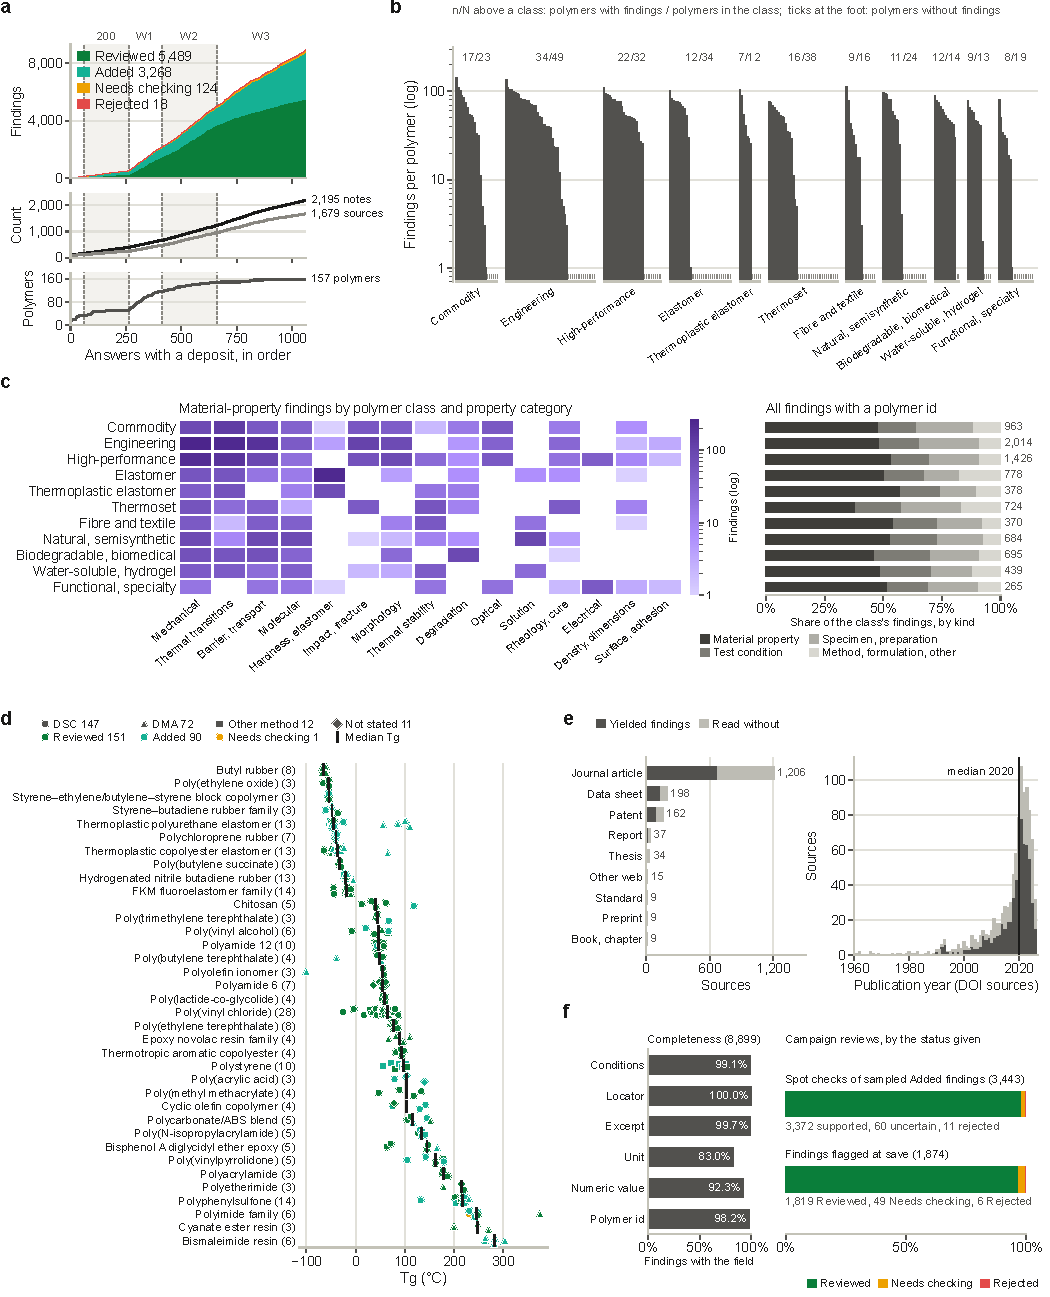
\includegraphics[width=\textwidth,height=0.62\textheight,keepaspectratio]{figures/fig3}
  \caption{The knowledge base as a polymer dataset (KF, 8,899 findings).
  (a) Growth over the 1,063 answers that deposited findings, in deposit order: findings stacked by status, source notes, distinct sources, and polymers with a finding; dashed lines mark the first answer under a new prompt or model, and shaded bands the 200-task run and wave 2.
  (b) Findings per polymer for all 274 polymers of the seed release, grouped by class and sorted within class (log scale); polymers without findings are ticks at the foot, and each label gives the polymers with findings over the polymers in the class.
  (c) Material-property findings by polymer class and property category (shade, log scale), and the share of each class's findings by kind.
  (d) Glass transition temperatures with one readable value for the 36 polymers with at least three, one point per finding, marked by method and colored by status, with each polymer's median.
  (e) Distinct sources by type, split into those that yielded findings and those read without yielding any, and the publication years of the 995 DOI sources known to Crossref.
  (f) Field completeness over all findings, and the outcomes of reviews during the build for spot-checked Added findings and for findings flagged when saved.}
  \label{fig:dataset}
\end{figure*}

The knowledge base grew to 8,899 findings, 2,195 source notes, and 1,679 distinct sources over the 1,063 answers that deposited anything, and its coverage is broad but uneven across polymer classes (Figure~\ref{fig:dataset}a,b).
The number of polymers with a finding rose quickly in the first stages and then leveled off at 157, as later questions returned to the polymers of the question bank.
Of the 274 polymers in the seed, 143 have at least ten findings and 90 have at least 50, and the ten best-covered polymers hold 13.1\% of the findings that carry a polymer identity.
The least-covered classes are elastomers (12 of 34 polymers with findings), functional and specialty polymers (8 of 19), and thermosets (16 of 38).
This pattern mostly reflects which polymers were asked about rather than which polymers the open literature describes.
Only 163 findings (1.8\%) lack a polymer identity.

Only half of the findings are material properties; the rest record how those properties were measured (Figure~\ref{fig:dataset}c).
Of all findings, 49.1\% are material properties, 21.6\% describe the specimen and its preparation, 18.4\% give a test condition, 7.6\% name a method, and 2.6\% give a formulation.
This split follows from the deposit rule, which saves the method and specimen details that accompany a value as findings in their own right, so that a later question can use the value with its conditions without reopening the source.
The material-property findings span 125 property classes and 1,389 polymer--property pairs.

Because each value keeps its method, the glass transition temperatures (Tg) in the store retain the spread that a single tabulated value would hide (Figure~\ref{fig:dataset}d).
The store holds 294 Tg findings with one readable temperature, measured by differential scanning calorimetry (DSC; 185), dynamic mechanical analysis (DMA; 78), other methods (12), or an unstated method (19), and 36 polymers have at least three such values.
Among the 15 polymers with both DSC and DMA values, the median DMA value exceeds the median DSC value in 11, and the median difference across the 15 is \SI{12.0}{\celsius}.
This is the direction expected, because a dynamic Tg taken from a mechanical loss peak at a finite frequency generally lies above the calorimetric value.\cite{Hutchinson2009Glass,GraciaFernandez2010Comparative}
Differences of more than \SI{40}{\celsius} in either direction, such as those for the thermoplastic polyurethane (\SI{+142}{\celsius}) and the polyolefin ionomer (\SI{-156}{\celsius}), are too large for a method offset and more likely compare different transitions, phases, or grades.
The store keeps each of these values with its source and conditions rather than reconciling them, which leaves the judgment to the question that uses them.

The sources are recent, largely open, and broader than journal articles, and the researcher's direct readings rarely failed review (Figure~\ref{fig:dataset}e,f).
Of the 1,679 distinct sources, 951 yielded findings; journal articles account for 1,206 sources, technical data sheets for 198, and patents for 162.
The DOI sources have a median publication year of 2020, and 62.4\% are open access by Crossref's indicator, proportions that we attribute to what the researcher can open rather than to the polymer literature as a whole.
Conditions, locators, and excerpts are present for 99.1\%, 100\%, and 99.7\% of findings.
Reviewers rejected 11 of the 3,443 Added findings sampled for spot checks during the build (0.3\%) and 6 of the 1,874 findings flagged for review when saved.
These rates are reviewer judgments, not a human audit, and a double review of 100 findings confirmed every Reviewed finding but overturned 12 of 28 rejections, mostly over wording (Section~S6).
A rejection is therefore a less reliable verdict than a confirmation.

%% ---------------------------------------------------------------------------------------------
\subsection{Saved Findings Make Questions near Past Work Cheaper}
\label{sec:memory}

\begin{figure*}
  \centering
  \singlespacing
  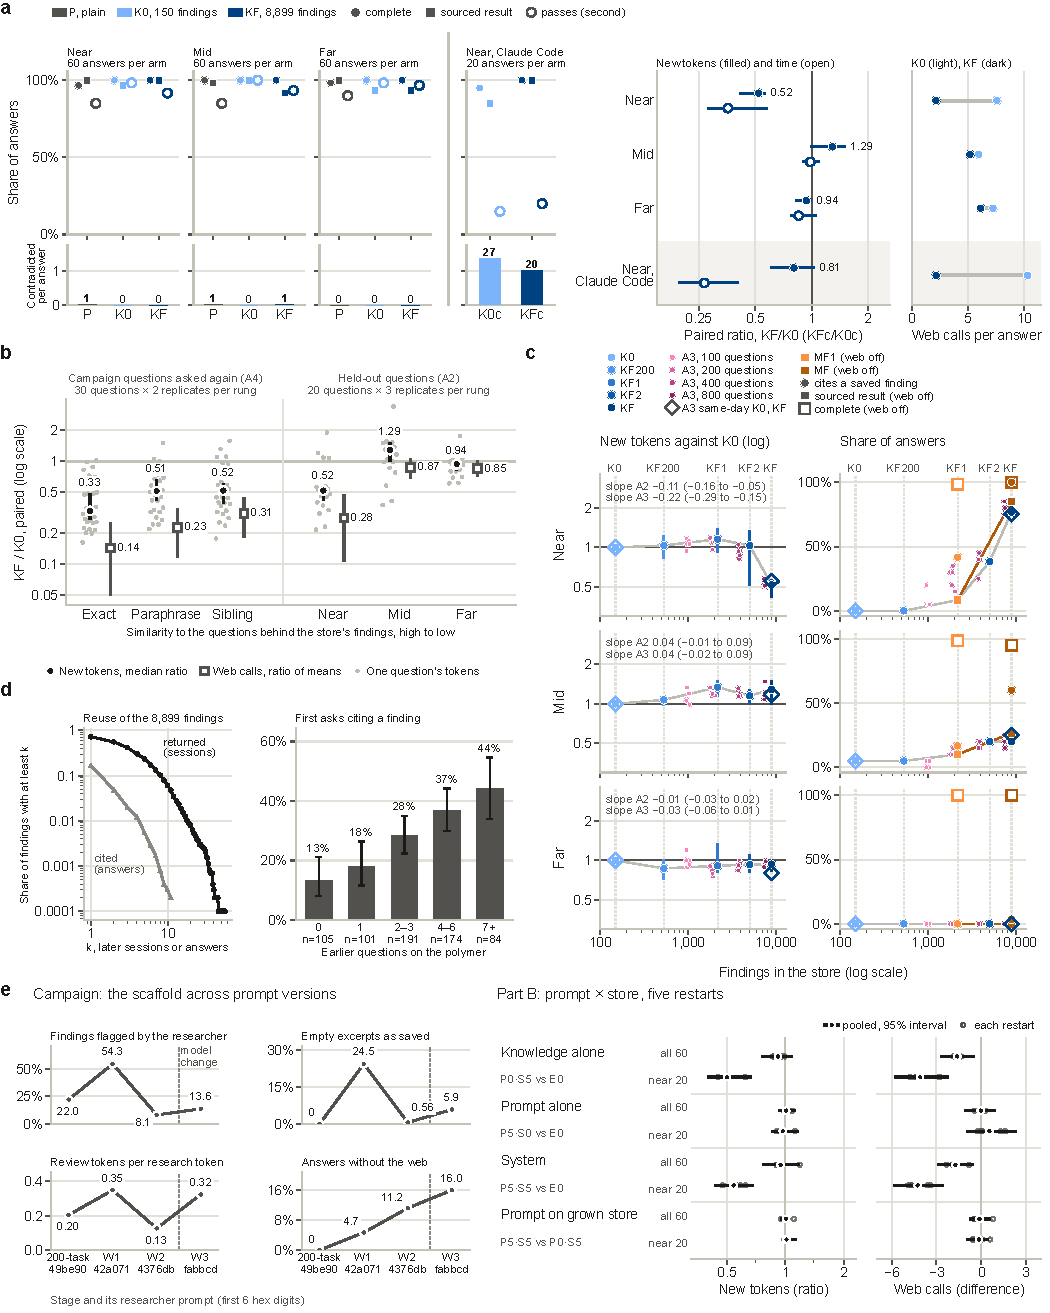
\includegraphics[width=\textwidth,height=0.6\textheight,keepaspectratio]{figures/fig4}
  \caption{Performance, reuse, scaling, and self-improvement.
  P is the plain session, K0 the researcher on the 150-finding store, and KF the researcher on the frozen knowledge base; token ratios are medians of paired per-question ratios with bootstrap 95\% intervals.
  (a) Memory ablation on 60 held-out questions (near, mid, and far; three replicates) and, in the fourth column, the 20 near questions answered on Claude Code: answers complete, with a sourced result, or passing (secondary), with contradicted statements (left); KF/K0 ratios of tokens and time (middle); and web calls per answer (right).
  (b) KF/K0 token ratios (filled) and web-call ratios (open) for campaign questions asked again exactly, reworded, or as siblings, and for the three held-out strata.
  (c) Tokens against K0 (left) and answers citing a saved finding or, with the web off, giving a sourced result (right), against store size for the cut stores (lines) and the resampled stores (marks).
  (d) Shares of findings returned by at least $k$ later searches or cited by at least $k$ later answers, and the share of campaign first questions citing a finding against the number of earlier questions on the polymer.
  (e) Measures targeted by prompt changes across the campaign's stages (left), and the restarts' prompt and store crossing (right), pooled (filled) and per restart (open).}
  \label{fig:performance}
\end{figure*}

Saved findings were widely retrieved, more narrowly cited, and reused more as a polymer's coverage grew (Figure~\ref{fig:performance}d).
Of KF's 8,899 findings, 72.7\% were returned by at least one later session's search and 16.7\% were cited by at least one later answer, and saved findings make up 63.2\% of the citations in campaign answers.
The share of campaign first questions citing a saved finding rises from 13\% for a polymer with no earlier campaign question to 44\% after seven or more.
We read the gap between retrieval and citation as the search doing its job, in that a session sees many candidate findings and cites the few that answer its question.

On held-out questions near past work, the full store roughly halved the researcher's cost without lowering source support (Figure~\ref{fig:performance}a).
Against the same researcher on K0, the researcher on KF used 0.52 (0.41--0.57) of the new tokens and 0.36 of the time on near questions, and its web calls fell from 7.6 to 2.1 per answer.
It answered 36 of its 60 near answers without the web, and 46 of them cited a saved finding.
Neither arm had a contradicted statement on near questions, and KF gave a sourced result in 60 near answers against K0's 58.
Across all three strata, each researcher arm with web access had at most two contradicted statements in 180 answers.

The saving does not extend to a covered polymer asked about from an unasked angle.
Mid questions cost more on KF than on K0 (1.29, 0.99--1.52), and far questions cost about the same (0.94, 0.82--1.00).
On mid questions KF and the two largest stores cut from it at earlier stages (Section~\ref{sec:coverage}) also gave a sourced result less often (53 to 55 of 60, against 60 on K0), which we did not predict.
We attribute the mid-question cost to findings about other properties of the same polymer, which the researcher reads without being spared any web search.
Against a plain web session of the same engine (P), the researcher on KF used 0.57 of P's tokens on near questions, whereas the researcher on K0 used more than P (1.23 on near questions).
The instructions to cite, label, and deposit therefore cost tokens that the store repays only where it covers the question.
The extended results, including the pass rates, the store answering alone with the web disabled, and a second engine reusing the store, are given in Section~S9.
The store also lowered the cost of a second engine: answering the near questions on Claude Code, the researcher cut its web calls from 10.3 to 2.1 per answer, but these answers were less well supported, so we claim the cost benefit of shared memory across engines and not parity of source support.

\subsection{Coverage, Not Store Size, Carries the Saving}
\label{sec:coverage}

The closer a question is to one already answered, the cheaper it is, but only an exact repeat is clearly cheaper than a new question on a saved topic (Figure~\ref{fig:performance}b).
Asked again on KF, 30 campaign questions cost 0.33 (0.27--0.49) of their K0 tokens as exact repeats, 0.51 (0.42--0.66) when reworded, and 0.52 (0.39--0.61) as siblings, the same as a held-out near question.
KF gave a sourced result at least as often as K0 on every rung but had more contradicted statements (seven against two over the three rungs).
Four of the seven repeat one wrong page number from a set of saved findings whose values are right but whose locator gives the wrong page of a data guide.
Review checks a value against its source but not the page, so the wrong locator passed review and reached every answer that reused those findings without the web.

Store size alone does not lower cost; coverage of the question's own topic does (Figure~\ref{fig:performance}c).
On stores cut from KF at earlier stages, near-question tokens fall with store size (within-question slope of log tokens on log findings $-0.108$, $-0.159$ to $-0.051$), while mid and far questions show no trend.
Twenty further stores, built by sampling the questions that made KF at random, separate the two effects.
With the presence of a near question's parent, the campaign question it was drawn from, in the model, a near question costs 0.45 (0.36--0.58) of its tokens when its parent is in the store, and the store's size adds nothing (log-findings coefficient 0.007, $-0.054$ to 0.068).
The share of near answers citing a saved finding tracks the parents present, with 8, 26, 38, and 80 of 100 answers citing one on stores of 100, 200, 400, and 800 questions that hold 8, 22, 40, and 93 of the 100 near parents.

Five independent restarts from an empty store reproduced both the saving and its dependence on coverage (Figure~\ref{fig:performance}e; Section~S10).
Each restart answered five rounds of 100 tasks drawn with its own random seed and built a store of 3,776 to 4,321 findings on 133 to 146 polymers (Figure~S1).
With the initial prompt, each restart's final store cut near-question tokens to 0.45 to 0.62 of the empty store's (pooled 0.50, 0.40--0.67), while far questions stayed flat in four of the five restarts.
A near question whose parent was in the store cost 0.47 (0.35--0.65) of the baseline, one whose parent had not yet been saved cost 1.29, and the store's size added nothing distinguishable from zero (Figure~S2).
Variance between restarts is negligible next to this effect, and contradicted statements did not rise with store size, with 25 in all 3,000 answers, 23 of them in answers that cited no saved finding.
We conclude that a store does not become better in general as it grows.
It becomes better at the topics that earlier questions covered, and a question on a new topic, or on a new angle of a covered polymer, pays the full cost of research.
For a polymer data resource, this argues for growing the store along the questions that researchers actually ask rather than by exhaustive harvesting.

%% ---------------------------------------------------------------------------------------------
\subsection{Provenance in Answers: Case Studies and Planted Errors}
\label{sec:cases}

\begin{figure*}
  \centering
  \singlespacing
  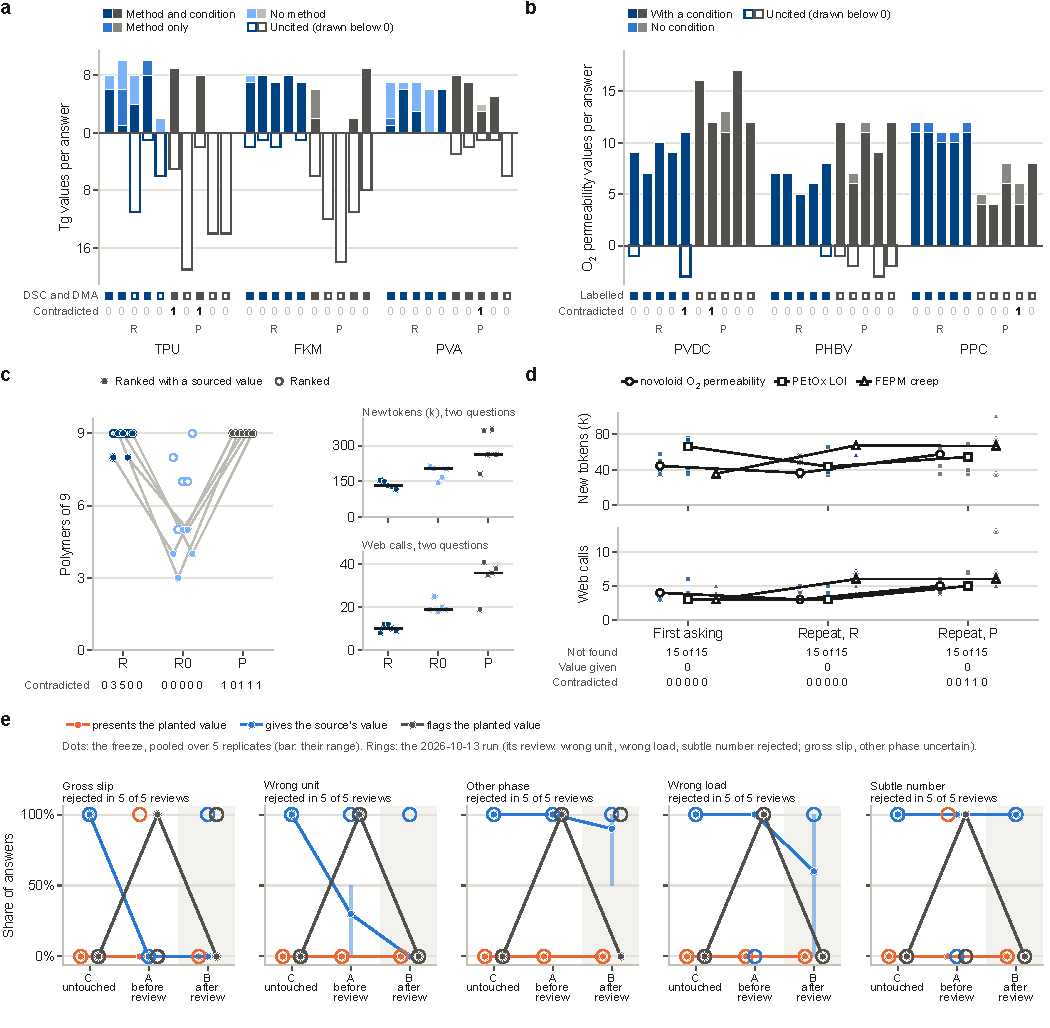
\includegraphics[width=\textwidth,height=0.6\textheight,keepaspectratio]{figures/fig5}
  \caption{Case studies and planted errors, five replicates each; R is the researcher on KF and P the plain session.
  (a) Tg of thermoplastic polyurethane (TPU), fluoroelastomer (FKM), and poly(vinyl alcohol) (PVA) and its dependence on method and conditions: sourced values per answer by whether they name a method and a condition, uncited values below zero, answers giving both DSC and DMA values (markers), and contradicted statements (digits).
  (b) Oxygen permeability of PVDC, PHBV, and PPC films: sourced values with and without a stated condition, uncited values below zero, and whether the explanation of the spread was labeled as interpretation.
  (c) Two rankings of nine polymers by oxygen permeability, also answered on an empty store (R0): polymers ranked with a sourced value and ranked at all, with tokens and web calls per replicate.
  (d) Three questions not expected to be answerable from open sources, asked first through the loop and then reworded to R and P: tokens and web calls.
  (e) Five planted wrong findings on the untouched store (C), before review (A), and after one review (B): shares of answers presenting the planted value as the source's, giving the source's value, or flagging the planted value (filled, pooled; bars, range), with an earlier run under the previous prompt (rings).
  Case counts were scored blind to the arm against rubrics written before any answer was read.}
  \label{fig:cases}
\end{figure*}

The case studies show how the provenance of saved findings changes an answer beyond its cost (Figure~\ref{fig:cases}; Section~S9).
Each was run five times by the researcher on KF beside the plain session, and case-specific counts were scored from the answer text by a session blind to the arm.
Asked for the Tg of thermoplastic polyurethane, fluoroelastomer, and poly(vinyl alcohol) and how it depends on method and conditions, the researcher gave 109 sourced values, 80 with their method and 72 also with a condition, and left 24 uncited, whereas the plain session gave 58 sourced values and left 122 uncited (Figure~\ref{fig:cases}a).
The researcher also gave both DSC and DMA values in 13 of 15 answers, against 9, at about half the tokens.
Asked why published oxygen permeabilities differ for three barrier films, both arms reported conflicting values with their conditions, but only the researcher labeled its explanation of the spread as its own interpretation, in 15 of 15 answers against none (Figure~\ref{fig:cases}b).
For two rankings of nine polymers by oxygen permeability, the researcher on KF ranked eight or nine with a sourced value in every replicate, against three to five on an empty store, with fewer tokens and web calls (Figure~\ref{fig:cases}c).
It was also the one arm with repeated contradicted statements, all in its own labeled interpretations, where it converted permeability units wrongly or stated orders that contradicted the values it had computed.
Saved knowledge supplied the values, and arithmetic across units remained the researcher's weak point.
Asked three questions that open sources are not expected to answer, every one of 45 answers said that no value was found (Figure~\ref{fig:cases}d).

Planted errors show both what review catches and what the researcher does with an unverified saved value (Figure~\ref{fig:cases}e).
Five Reviewed findings in a copy of KF were replaced by wrong versions filed as Added, and each plant's question was answered before and after one normal review.
The reviewer rejected all 25 planted findings across five replicates.
Before review, no answer asserted a planted value as verified, and all 50 doubted it, as the prompt instructs for an Added finding whose excerpt does not show its value.
That count is generous, because 9 of the 10 answers about a decimal slip still attributed the planted \SI{12.27}{\mega\pascal} to the source's table while calling it provisional.
After review, with the plant rejected and hidden from search, no answer repeated a planted value, but only 25 of 50 gave the source's value; most said that the value could not be confirmed and did not reopen the source.
Doubt about a saved value is therefore necessary but not sufficient, and the behavior that matters, reopening the cited source, was inconsistent.

%% ---------------------------------------------------------------------------------------------
\subsection{Reflection on the Records: Revising the Prompt}
\label{sec:improve-results}

Revising the researcher's prompt from the loop's records found plausible edits but no measurable gain (Figure~\ref{fig:performance}e; Sections~S7 and S10).
During the campaign, a maintainer session revised the prompt after each wave, and each measure that a change targeted moved after it; the share of findings saved with an empty excerpt, for example, fell from 24.5\% to 0.56\%.
These changes were confounded with new questions and a new model, so the restarts tested the automated heuristic instead.
Across the five restarts, the improver proposed 25 edits and the rule adopted 11, one to three per restart (Figure~S1).
The adopted edits partly converge: scoping a claim that a source lacks a detail to the part that was read, answering from the store when its findings cover the question, reopening a cited finding's own source for a missing detail, and repeating knowledge searches less often were each adopted in two restarts.
Nevertheless, the final prompts changed cost by nothing measurable, either on the empty store (1.01, 0.93--1.13) or on the grown store (1.01, 0.94--1.04), and on the empty store they gave a sourced result less often (277 against 295 over the five restarts).

We see two reasons in the records.
The development set barely touches a restart's store, since 0 to 4 of 30 development answers per arm cite a saved finding, so edits aimed at reuse were judged on questions that their store could not inform.
In addition, 11 of the 12 rejections for completeness or sourced results were decided by a single answer of 30, so the rule cannot separate a useful edit from noise.
A larger development set drawn from each store's own topics is the obvious next test of this heuristic.

\subsection{Reflection on the Records: Refining the Ontology}
\label{sec:ontology}

\begin{figure*}
  \centering
  \singlespacing
  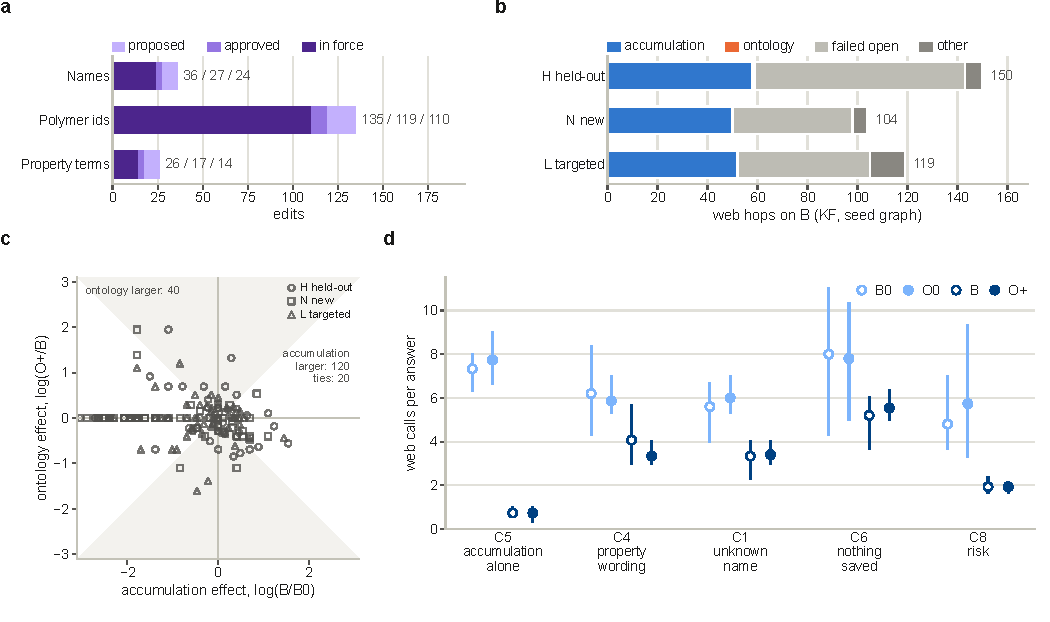
\includegraphics[width=\textwidth,height=0.5\textheight,keepaspectratio]{figures/fig6}
  \caption{Refining the ontology from answer traces on the frozen knowledge base.
  B0 is the researcher on K0 with the seed ontology, B on KF with the seed ontology, and O0 and O+ the same stores with the refined ontology.
  (a) Edits proposed by the curator, approved by the reviewer, and in force after the replay's drop step, by type (names, polymer-identity annotations, and property terms; 197, 163, and 148 in all).
  (b) B's 373 web hops on the 180 withheld questions by what they reached, for each question set: limited by accumulation (a source the store did not hold, a detail it had not saved, or a finding saved since), avoidable by the ontology (a finding the store held that no earlier search returned), failed page opens, and other hops (repeats and searches that ended without an open).
  (c) The accumulation effect, log(B/B0), against the ontology effect, log(O+/B), in web steps (web calls plus one) for each withheld question, marked by set; the accumulation effect is the larger in 120 questions (white) and the ontology effect in 40 (shaded), with 20 ties.
  (d) Case studies selected by mechanism before any refined answer was read: web calls per answer (mean over three questions and five replicates; bars, range of replicate means) on B0, O0, B, and O+; the B0 and O0 arms of the unknown-name case are also the case of the ontology without knowledge.}
  \label{fig:ontology}
\end{figure*}

In the experiments above the ontology never changed, because graph releases were built from the wiki seed alone and reflection edited only the prompt.
We therefore tested the second heuristic separately, holding KF's findings and the prompt fixed and changing only the ontology (Section~S11).
Mining 1,329 recorded answers and KF's stored findings found 750 misses, 587 of them in 230 answers: 297 polymer names that the ontology did not resolve, 163 of them on stored findings without a polymer identity, 426 late finds, in which an answer cited a finding that its first search for that polymer and property had not returned, and 27 findings saved again because a search had missed them.
From these, the curator proposed 197 edits, the reviewer approved 163, and 148 remained in force after assembly and the drop step, namely 24 names, 110 polymer-identity annotations, and 14 property-term edits forming nine terms (Figure~\ref{fig:ontology}a).
The reviewer rejected, among others, blend findings filed under one polymer and names broader than their polymer, and the drop step removed edits that crowded relevant results out of the first ten, such as two spelling variants of PEEK and broad mechanical-property terms.
No polymer, family link, or source link was proposed, and the traces surfaced only one candidate pair of sources.
In sample, the edits in force fixed 197 of the 750 misses.

On 180 withheld questions, the refined ontology improved lookup but not answers.
The questions comprised the 60 held-out questions above, 60 new questions from the campaign generator, and 60 targeted at names the store does not use, at family-level questions, and at values with their method and specimen.
Offline, recall of the relevant findings in the first ten results rose from 0.90 to 0.92, with 84 relevant results gained and 45 lost (2.5\%), and the largest gain, on mid questions (pooled recall 0.70 to 0.86), came from property terms that reach findings worded otherwise.
End to end, the researcher on KF with the refined ontology (O+) used 0.99 (0.95--1.02) of the tokens and 0.97 (0.89--1.06) of the web calls of the same researcher with the seed ontology (B), with six contradicted statements in each arm.
On the same questions, accumulation alone, B against the researcher on K0 (B0), cut tokens to 0.88 (0.73--0.99) and web calls to 0.67 (0.56--0.78).

The traces explain why the ontology mattered so little (Figure~\ref{fig:ontology}b,c).
Of B's 373 web hops, 160 were limited by accumulation, reaching a source the store did not hold, a detail it had not saved, or a finding saved since the answer ran, and 185 were page opens that failed.
Only one reached a finding that the store held but no earlier search had returned, and of 44 such store searches, none became reachable with the refined ontology.
Per question, the accumulation effect was the larger in 120 of 180 questions and the ontology effect in 40, with 20 ties.
The case studies, chosen by mechanism before any refined answer was read, show the same ordering (Figure~\ref{fig:ontology}d).
Where the store already covered the topic, saved knowledge removed about 90\% of web calls (7.33 to 0.73 per answer) and the refined ontology added nothing.
Where a question worded a property differently from the store, the refined ontology had its largest effect, 0.87 of the tokens and 0.92 of the web calls.
For a polymer name the seed lacked, the researcher reached the same findings by searching other names, so the new name changed nothing; where nothing relevant had been saved, the refined ontology changed nothing (0.98 of the tokens); and an edit that crowded another polymer's findings into the first ten did no visible harm in answers.

We conclude that trace review finds real lookup failures, chiefly spelling variants of polymer names, findings without a polymer identity, and property synonyms, and fixes some of them, but the researcher already recovers from most of them by searching again.
On these questions, cost is set by what has been saved rather than by how it is indexed.
This test was one round by one curator engine on a store whose topics were already well covered, and the curator could fix only what the traces showed: the trade names used by the targeted questions never appeared in them, and family links missing from the graph were never surfaced as misses.
The approved edits are not yet part of the released ontology.
Where new polymers, names, and property vocabularies enter the store, as in a new synthesis campaign or a new polymer class, the same heuristic may have more to fix, and that is where it should be tested next.

%% ---------------------------------------------------------------------------------------------
\section{Conclusions}
\label{sec:conclusions}

We've developed and benchmarked OOPC, an open-source harness compatible with frontier ai models that accumulates polymer knowledge as it is used.
OOPC implements a memory system that stores source-backed findings against an ontology of polymer identities and properties, reviews findings as they are incorporated into the knowledge base, and periodically updates the storage ontology based on research traces within the harness.
Over a campaign of 1,092 tasks, the harness build a knowledge base of 8,899 findings, from 1,679 sources (open-source publications or patents) involving 157 unique polymers.
Durable gains were reproduced across fresh restarts of the knowledge base, on withheld tasks of varying overlap with prior research tasks, and between claude and openai families of models.
The clearest gains involved the harness getting better at tasks where prior findings had at least partial bearing; on completely new tasks, parity with the underlying models was generally obtained.

A critical aspect of this work is that the user owns the memory system and can share or export it as they see fit.
All findings and the ontology are stored locally on the user's system, allowing research groups or other organizations the ability to pool a knowledge base across tasks or to adapt the memory system to their needs.
We also demonstrate the interoperability of the memory by switching between claude and codex here, with the findings extracted from tasks performed by one enriching the other.
More tests were run with codex owing to the availability of multiple resets over the project period being available to the author, so most prompts and hyperparameter tuning are likely to favor codex at the initial release; nevertheless, the opus-5.5 performance on a mostly codex extracted knowledge base suggests that the knowledge base is interoperable.

The use of the reflection mechanism to automatically improve the ontology is the least investigated aspect of the harness.
In our tests we expected that reflection-based ontology augmentation could lead to a reduced number of hops to look of the findings relevant to a task, or improved token efficiency, or reduced inconsistencies for findings.
However, after the full campaign we observed a near zero inconsistency rate in withheld tasks and high token and lookup efficiency that left little room to demonstrate the ontology improvement.
We hypothesize that the benefits of ontology refinment will manifest on a) longer running research tasks with more steps (e.g., synthesis or lifecycle analysis), or b) tasks that involve different finding usage patterns (e.g., solving inverse problems rather than forward problems), or c) at extremely high levels of accumulation where subtle differences in the salience of findings matter, or d) tasks that are budget limited (e.g., where number of hops or lookups are strongly constrained relative to task complexity), or e) vocabulary and usage shifts with time that make the ontology ill suited to ongoing accumulation.
None of these were directly tested here as they justify separate study.
Nevertheless, in the present experiments the ontology edits showed no loss in performance in general, and even a marginal positive effect by raising search recall by identifying uncommon property names when registering new findings.

Several limitations of the current study should be highlighted.
Accuracy in the current studies were entirely judged by supporting sources and self-consistency by independently instantiated ai models.
This leaves aside the question of reconciling inaccurate data in the published works that were ingested into the knowledge base.
The experiments performed here were of relatively limited scope owing to token costs.
We hope that by open-sourcing the harness that it is more broadly adopted and tested.
Lastly, the knowledge base inherits the biases of the open-source literature owing to the general inaccessibility of the latest research in many publication venues. Unfortunately, the literature that is freely accessible isn't necessarily the most accurate or state-of-the-art knowledge available to the field.

%% ---------------------------------------------------------------------------------------------
\begin{suppinfo}
%The Supporting Information is available free of charge at \tbd{DOI}.
Detailed methods: the seed ontology and data model, with counts of the seed and knowledge base (Table~S1); polymer resolution; the researcher session and the released two-turn session; deposit and review; search and reuse; the build of the knowledge base; prompt improvement; answer checking and measures; the controlled experiments; the restarts from an empty store (Figures~S1 and S2); the ontology refinement (Tables~S2--S4); the confirmation run on the released code (Table~S5); the records analyses; statistics; run accounting; and the researcher's prompt (PDF).
\end{suppinfo}

\section{Data Availability}
The seed release (\ident{oopc-6ad56d8b354d053bcc3cf3a1}) and the knowledge snapshot (\ident{oopc-knowledge-db1fc22ca88a0c0b45b9218b}) are available at \tbd{repository and DOI}.
The snapshot carries each finding's statement, material, property, value, unit, conditions, polymer identifier, source, locator, status, and review verdict with its reason, together with every source note.
Structured fields are released under CC0-1.0, and finding statements and notes under CC BY 4.0.
The code is available at \url{https://github.com/bsavoie/open-ontology-of-polymer-chemistry} under the Apache-2.0 license, with the frozen revisions used here tagged \code{study-freeze-2} (the knowledge base experiments and restarts), \code{study-freeze-3} (the ontology refinement), and \code{study-freeze-4} (version 0.13.0 and the confirmation run).

\begin{acknowledgement}
The abstract and conclusions were written by Brett, the rest of the manuscript is the result of multiple drafts between Opus 5.5 and 6.5-Sol with light editing from Brett.
Figures 1--6 and the table-of-contents graphic were drawn by scripts written by Claude Opus 5.5.
I appreciate conversations with Chris Sweet and Charles Vardeman about llmwiki memory systems that influenced the original open polymer wikipedia project (\url{https://github.com/bsavoie/wiki-of-open-polymer-data}) that was used to seed OOPC.
\end{acknowledgement}

\bibliography{refs}

\end{document}
